\documentclass[11pt,a4paper]{ltjsarticle}
% Compile with LuaLaTeX

\usepackage{luatexja}
\usepackage{graphicx}
\usepackage{hyperref}
\usepackage{amsmath,amssymb,mathtools}
\usepackage{xcolor}
\usepackage{float}
\usepackage{booktabs}
\usepackage{enumitem}
\usepackage{geometry}

\geometry{margin=22mm}

% =========================
% Colour scheme (WRN/rule.txt)
% =========================
\definecolor{SciBlue}{HTML}{1C3177}      % Primary
\definecolor{DeepIndigo}{HTML}{4B0082}   % Accent
\definecolor{MistLavender}{HTML}{E8EAF1} % Pale
\definecolor{MidnightInk}{HTML}{101426}  % Dark
\definecolor{OpticWhite}{HTML}{FFFFFF}   % Background

\color{MidnightInk}

\newcommand{\sectionblock}[1]{%
  \vspace{4mm}
  {\large\textbf{\textcolor{SciBlue}{#1}}}
  \vspace{2mm}

}

\newcommand{\todo}[1]{\textcolor{red}{#1}}

\title{Weekly Report (Pre-registration): Decision Rule for the Zero-Contrast Contour N1}
\author{Risei Abe (Institute of Science Tokyo)}
\date{Week: 2026/08/31 -- 2026/09/06}

\begin{document}

\maketitle

\noindent
{\small\textcolor{SciBlue}{\textbf{Notation}}: the shot-noise sensitivity of CW-ODMR is \(\eta=\Delta\nu/(C\sqrt{R})\), where \(C\) is the resonance \emph{contrast} (a measured quantity), \(R\) the photon count rate and \(\Delta\nu\) the linewidth. For power-law responses \(C=(1+\rho)^{-c}\), \(R=\Gamma_p(1+\rho)^{-s}\), \(\Delta\nu=(1+\rho)^{w}\) with \(\rho=\Gamma_p/\Gamma\), the lower-case \(c,s,w\) are the \emph{exponents}, and Theorem G states that they enter \(\eta\) only through the single scalar \(E\equiv 2c+s+2w\). What changes sign below is the upper-case \(C\), not the exponent \(c\).}

% =========================================================
% 1. Question / Purpose
% =========================================================
\sectionblock{Question}

Can a numerical decision rule for identifying the zero-contrast contour N1 as a dark line be fixed before any wide-field ODMR image is opened?

% =========================================================
% 2. Hypothesis
% =========================================================
\sectionblock{Hypothesis}

Along the contour where \(C\) crosses zero, \(\eta=\Delta\nu/(C\sqrt{R})\) diverges (it is \(C\) that reverses sign, not \(\eta\)), so a dark line of vanishing ODMR contrast should appear in the wide-field image.

% =========================================================
% 3. Evidence / Interpretation
% =========================================================
\sectionblock{Evidence / Interpretation}

\begin{itemize}[leftmargin=8mm]
  \item Bhattacharyya \S6.3 reports a complete inversion of the resonance peak above 60 GPa in both [100] and [110], universally across sample geometries [1]. If \(C\) passes from positive to negative, a \(C=0\) contour must lie in between.
  \item Figure~\ref{fig:width} fixes what the decision rule has to specify. The apparent width of the dark line is not a property of the contour but of the detection threshold: for a contrast crossing zero with slope \(|\mathrm{d}C/\mathrm{d}x|\), a threshold of \(0.5\,C_0\) gives a line of width \(1.0\,L\) and a threshold of \(0.2\,C_0\) a line of width \(0.4\,L\), where \(L=C_0/|\mathrm{d}C/\mathrm{d}x|\). A rule that names a width without naming the threshold is empty.
\end{itemize}

\begin{figure}[H]
  \centering
  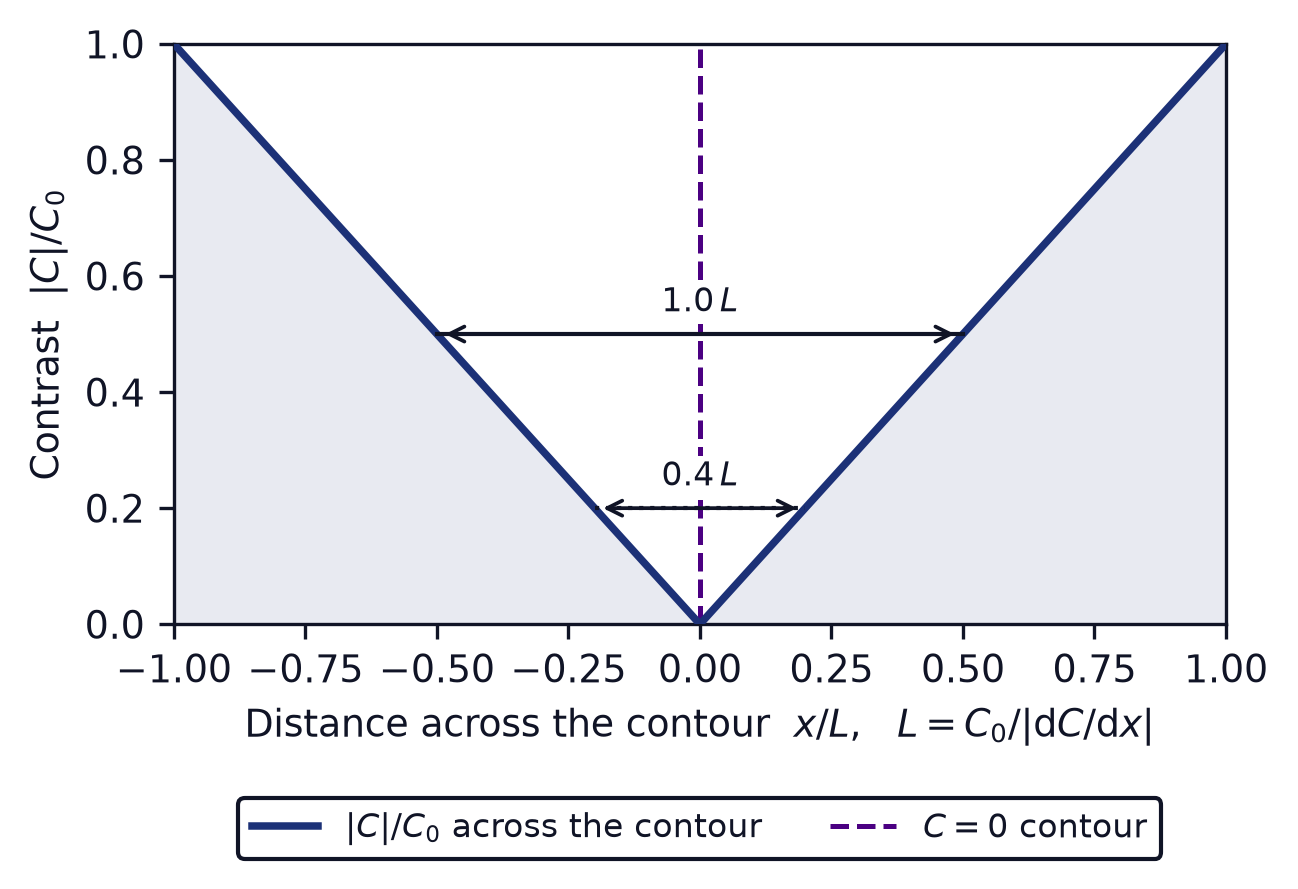
\includegraphics[width=0.58\linewidth]{image/wrn_zero_contrast_width.png}
  \caption{Contrast magnitude across the \(C=0\) contour, in units of the crossing
  scale \(L=C_0/|\mathrm{d}C/\mathrm{d}x|\), for a locally linear crossing. The two arrows
  give the apparent line width at detection thresholds \(0.5\) and \(0.2\). Schematic:
  the crossing slope itself is not predicted by the theory and must be measured.}
  \label{fig:width}
\end{figure}

% =========================================================
% 4. Gap / Failure
% =========================================================
\sectionblock{Gap / Failure}

\begin{itemize}[leftmargin=8mm]
  \item The threshold, the required continuity of the line and the crossing scale \(L\) are not yet fixed numerically, so there is still no criterion separating the feature from instrumental non-uniformity (illumination gradients, the gasket edge, stress concentration). Opening the figure without one would make the judgement post hoc.
  \item The reported inversion occurs in [100]/[110] and in the gasket region of [111] cut anvils, which is \emph{outside} the domain in which we claim wavelength optimisation ([111] cut culet, [111] NV group, inside the sample chamber). N1 must therefore be stated as a prediction about the exterior of that domain.
\end{itemize}

% =========================================================
% 5. Next Step
% =========================================================
\sectionblock{Next Step}

Fix and register the three numbers the rule needs --- detection threshold, minimum line continuity, and the expected range of \(L\) --- and only then open Fig.~6.7(b).

% =========================================================
% 6. References
% =========================================================
\sectionblock{References}

\begin{enumerate}[leftmargin=8mm]
  \item P. Bhattacharyya, \textit{Principle and applications of quantum metrology in diamond anvil cells using the Nitrogen Vacancy color center}, PhD thesis, University of California, Berkeley (Fall 2022), \S6.3 and Fig.~6.7(b).
  \item A. Dr\'eau \textit{et al.}, ``Avoiding power broadening in optically detected magnetic resonance of single NV defects for enhanced dc magnetic field sensitivity,'' \textit{Phys. Rev. B} \textbf{84}, 195204 (2011). Literature grounding for the exponent \(E=3\) of Theorem G.
\end{enumerate}

\end{document}
